\documentclass[a4paper,12pt]{article}
\usepackage{graphicx}
\usepackage[a4paper,margin=1in]{geometry}
\usepackage{titlesec}
\usepackage{hyperref}
\usepackage{amsmath}    % For math environments and symbols
\usepackage{amssymb}    % For \mathbb and other math symbols
\usepackage{amsfonts}   % Additional math fonts
\usepackage[backend=biber,style=numeric,sorting=none]{biblatex}

\addbibresource{references.bib} % Add references.bib with the appropriate entries

% Title format
\titleformat{\section}{\large\bfseries}{\thesection}{1em}{}

% Title settings
\title{
    \includegraphics[scale=0.4]{Cam_logo_bw.png}\\
    \vspace{0.5cm}
    C1 Research Computing - Coursework Assignment
}
\author{Raunaq Rai (rsr45@cam.ac.uk)\\
    Data Intensive Science, Department of Physics, University of Cambridge
}
\date{18 December, 2024 \\ \vspace{0.2cm} {\small Word Count: 2959}}

\begin{document}

\maketitle

\section*{Introduction}
This report details the development and implementation of a Python package, \texttt{dual\_autodiff}, designed for automatic differentiation using dual numbers. The package computes derivatives efficiently while supporting mathematical operations such as trigonometric, logarithmic, and exponential functions.

The approach builds on the concept of forward-mode automatic differentiation, which is essential in fields like optimisation, computational physics, and machine learning. This technique traces its roots to the foundational work by Wengert~\cite{wengert1964automatic}, who introduced a systematic way to compute derivatives using intermediate variables. More recently, Baydin et al.~\cite{baydin2018automatic} surveyed the use of automatic differentiation in machine learning, emphasising its importance in training deep neural networks.

To enhance performance, a Cython-optimised version, \texttt{dual\_autodiff\_x}, was also developed. This document covers the mathematical principles behind dual numbers, and the implementation details of the package.

The structure of this report follows that of the coursework problem sheet.

\section*{Theoretical Background}

Dual numbers can be defined as truncated Taylor series of the form:
\begin{equation}
    x = v + \dot{v}\epsilon,
    \label{eq:dual_number_form}
    \end{equation}
where \(v, \dot{v} \in \mathbb{R}\), and \(\epsilon\) is a nilpotent number such that \(\epsilon^2 = 0\) and \(\epsilon \neq 0\). Here:
\begin{itemize}
    \item \(v\): Represents the \textit{primal value}.
    \item \(\dot{v}\): Represents the \textit{derivative value}.
\end{itemize}

As explained by Baydin et al.~\cite{baydin2018automatic}, arithmetic operations with dual numbers align naturally with symbolic differentiation principles:
\begin{equation}
    (x_1 + \dot{x}_1\epsilon) + (x_2 + \dot{x}_2\epsilon) = (x_1 + x_2) + (\dot{x}_1 + \dot{x}_2)\epsilon,
    \label{eq:dual_addition}
    \end{equation}
    
    \begin{equation}
    (x_1 + \dot{x}_1\epsilon)(x_2 + \dot{x}_2\epsilon) = x_1x_2 + (x_1\dot{x}_2 + \dot{x}_1x_2)\epsilon,
    \label{eq:dual_multiplication}
    \end{equation}
    
Automatic differentiation uses dual numbers to compute derivatives efficiently. For a function \(f(x)\), substituting \(x = v + \dot{v}\epsilon\) yields:
\begin{equation}
    f(x) = f(v + \dot{v}\epsilon) = f(v) + f'(v)\dot{v}\epsilon,
    \label{eq:dual_function}
    \end{equation}
    
The derivative \(f'(v)\) is embedded in the coefficient of \(\epsilon\), enabling evaluation of function values and derivatives.

This principle extends to composite functions via the chain rule:
\begin{equation}
    f(g(v + \dot{v}\epsilon)) = f(g(v)) + f'(g(v))g'(v)\dot{v}\epsilon,
    \label{eq:composite_function}
    \end{equation}
    
    \section{Project Structure and Packaging}

    \subsection{Repository Organisation}
    The repository adheres to established best practices for Python projects to ensure clarity, maintainability, and modularity. Below is an overview of its structure:
    
    \subsubsection{Top-Level Directory}
    The top-level directory organises the project as follows:
    \begin{itemize}
        \item \textbf{\texttt{dual\_autodiff/}}: Core implementation, including modules like \texttt{dual.py}, \texttt{functions.py}, and \texttt{base.py}.
        \item \textbf{\texttt{dual\_autodiff\_x/}}: Cythonised implementation of the package for enhanced performance, including \texttt{.pyx} source files and compiled \texttt{.so} binaries.
        \item \textbf{\texttt{tests/}}: Unit tests for core modules. Use the \texttt{pytest} command to run the tests.
        \item \textbf{\texttt{docs/}}: Documentation files, including Sphinx configurations and example notebook.
        \item \textbf{\texttt{report/}}: LaTeX report and related files.
        \item \textbf{\texttt{dist/}}: Package distribution files (wheel and source archives).
        \item \textbf{\texttt{build/}}: Temporary build files.
        \item \textbf{\texttt{pyproject.toml}}: Modern Python project configuration.
        \item \textbf{\texttt{requirements.txt}}: Python dependencies.
        \item \textbf{\texttt{environment.yaml}}: Conda environment definition.
        \item \textbf{\texttt{README.md}}: Project overview and instructions.
        \item \textbf{\texttt{LICENCE}}: Contains the MIT License under which the project is distributed.
    \end{itemize}

    \section{Building and Installing the Package}

    The \texttt{pyproject.toml} file is used to manage the configuration and metadata of the project. The key sections are described below:
    
    \begin{itemize}
        \item \texttt{[build-system]}: Specifies the tools required to build the package, including:
        \begin{itemize}
            \item \texttt{setuptools}: For packaging and distribution.
            \item \texttt{wheel}: For building wheel distributions.
            \item \texttt{setuptools\_scm}: For dynamic versioning based on the repository's state.
            \item \texttt{build}: A modern tool for building Python packages.
        \end{itemize}
    
        \item \texttt{[project]}: Contains essential project metadata, including:
        \begin{itemize}
            \item \textbf{Name:} \texttt{rsr45\_dual\_autodiff}.
            \item \textbf{Description:} \textit{A Python package for forward-mode automatic differentiation using dual numbers}.
            \item \textbf{Author:} \texttt{Raunaq Rai} (\texttt{rsr45@cam.ac.uk}).
            \item \textbf{License:} \texttt{MIT License}, specified in the \texttt{LICENCE} file.
            \item \textbf{Dependencies:} 
            \begin{itemize}
                \item \texttt{numpy>=1.20.0}: For numerical computations.
                \item \texttt{pytest>=6.0}: For unit testing.
                \item \texttt{argparse}: For command-line interface support.
            \end{itemize}
            \item \textbf{Python Version:} Requires Python 3.9 or higher.
            \item \textbf{Keywords:} \textit{automatic differentiation, dual numbers, forward-mode}.
            \item \textbf{URLs:} Link to the gitlab repository.
        \end{itemize}
    
        \item \texttt{[project.scripts]}: Defines a command-line interface entry point for the package. The \texttt{dual\_autodiff} command is linked to \texttt{dual\_autodiff.cli:main}, enabling users to interact with the package via the terminal.
    \end{itemize}
    
    This configuration ensures that the package is documented, modular, and easy to build, install, and distribute. Using \texttt{pyproject.toml} aligns the project with modern Python packaging standards, making it accessible to a wide range of users and developers.
    

    \section{Implementation of Dual Numbers and Operations}

    The \texttt{dual.py} file implements the \texttt{Dual} class, the core of the \texttt{dual\_autodiff} package. This class defines dual numbers and supports operations such as addition, subtraction, multiplication, and division.
    
    \subsection{Arithmetic Operations}
    The \texttt{Dual} class simplifies arithmetic operations by overriding standard operators such as \texttt{+}, \texttt{-}, \texttt{*}, and \texttt{/}. This allows \texttt{Dual} objects to be used just like regular numbers.
    
    \subsection{Mathematical Functions}
    The \texttt{Dual} class also implements important mathematical functions such as:
    \begin{itemize}
        \item Trigonometric functions (\texttt{sin}, \texttt{cos}, \texttt{tan}).
        \item Exponential and logarithmic functions (\texttt{exp}, \texttt{log}).
        \item Hyperbolic functions (\texttt{sinh}, \texttt{cosh}, \texttt{tanh}).
        \item Square root (\texttt{sqrt}).
    \end{itemize}
    
    \subsection{Error Handling and Special Cases}
    The \texttt{Dual} class ensures that mathematical operations like \texttt{log} and \texttt{sqrt} are only applied within valid domains, raising appropriate errors when encountering invalid inputs.
    
    \subsection{Utility Functions}
    
    To enhance usability and simplify mathematical operations, two utility modules are provided as part of the package:
    
    \begin{itemize}
        \item \texttt{functions.py}: This module provides aliases for commonly used mathematical functions, such as \texttt{sin}, \texttt{cos}, \texttt{log}, and \texttt{sqrt}. 
        \begin{verbatim}
        from dual_autodiff.functions import sin, cos, log
        x = Dual(2, 1)
        result = sin(x) + log(x)
        \end{verbatim}
    
        \item \texttt{base.py}: This module includes helper functions to streamline operations on \texttt{Dual} instances:
        \begin{itemize}
            \item \texttt{is\_dual\_instance(value)}: A utility function that checks whether a given value is an instance of the \texttt{Dual} class. 
            \item \texttt{ensure\_dual(value)}: A function that wraps a non-\texttt{Dual} value into a \texttt{Dual} object with its derivative initialised to zero.
        \end{itemize}
    \end{itemize}
    
    \section{Making the Code into a Package}

    To build and install the package, we made use of the \texttt{pyproject.toml} file for configuration, the \texttt{requirements.txt} file for dependencies, and the structured organisation of the project.

    
    \subsection{Steps to Build and Install the Package}
    The package was built and installed as follows:
    \begin{itemize}
        \item \textbf{Install Build Tools:} Required tools like \texttt{setuptools} and \texttt{wheel} were installed using:
        \begin{verbatim}
        pip install build
        \end{verbatim}
        \item \textbf{Build Distributions:} Source and wheel distributions were created using:
        \begin{verbatim}
        python -m build
        \end{verbatim}
        The outputs (\texttt{.tar.gz} and \texttt{.whl}) were saved in the \texttt{dist/} directory.
        \item \textbf{Editable Installation:} The package was installed in editable mode using:
        \begin{verbatim}
        pip install -e .
        \end{verbatim}
        This allows changes to the source code to be directly reflected without reinstallation, streamlining development and testing.
    \end{itemize}
    

\subsection{Publishing to PyPI}

To make the \texttt{dual\_autodiff} package publicly available, it was uploaded to the Python Package Index (PyPI). The following steps outline the publishing process and installation instructions.


\begin{enumerate}
    \item \textbf{Create Distributions:}
    Build source and wheel distributions as done previously:

    \item \textbf{Upload to PyPI:}
    Use \texttt{twine} to securely upload distributions.
    
    Authentication with PyPI credentials was required.

    \item \textbf{Verify Upload:}
    \url{https://pypi.org/project/rsr45-dual-autodiff/}
\end{enumerate}

Install the package via \texttt{pip}:
\begin{verbatim}
pip install rsr45-dual-autodiff
\end{verbatim}

\section{Differentiating a Function}

\subsection{Function Definition}
The target function for differentiation is:
\begin{equation}
    f(x) = \log(\sin(x)) + x^2 \cos(x),
    \label{eq:function_definition}
    \end{equation}
    
The derivative of this function, computed analytically, is:
\begin{equation}
    f'(x) = \frac{\cos(x)}{\sin(x)} -x^2 \sin(x) + 2x \cos(x),
    \label{eq:function_derivative}
    \end{equation}
    

\subsection{Using Dual Numbers for Differentiation}
To compute \(f'(x)\) at \(x = 1.5\) using dual numbers:
\begin{itemize}
    \item Represent \(x\) as a dual number: \(x = 1.5 + 1\epsilon\), where the real part is \(1.5\) and the dual part represents the derivative.
    \item Substitute \(x\) into \(f(x)\) and use the dual number arithmetic to compute \(f'(x)\) from the dual part of the result.
\end{itemize}

\subsection{Results}

\subsubsection{Using Dual Numbers}
The function \(f(x)\) and its derivative \(f'(x)\) were computed at \(x = 1.5\) using dual numbers. The results are as follows:
\[
f(1.5) = 0.15665054756073515, \quad f'(1.5) = -1.9612372705533612
\]

\subsubsection{Using Manual Computation}
The analytical expression for \(f(x)\) and \(f'(x)\) was used to compute the same values at \(x = 1.5\). The results are:
\[
f(1.5) = 0.15665054756073515, \quad f'(1.5) = -1.9612372705533614
\]

\subsubsection{Comparison}
The results obtained using dual numbers closely match the analytically computed values, confirming the correctness of the dual number implementation. The slight discrepancy in the derivative (\(2 \times 10^{-16}\)) is attributed to double numerical precision limitations inherent to computers. As explained by Kahan~\cite{kahan1997ieee754}, floating-point numbers are represented using a finite number of bits under the IEEE (Institute of Electrical and Electronics Engineers) 754 standard, resulting in small rounding errors during arithmetic operations. While these errors are negligible for most practical purposes, they can accumulate in complex calculations, causing slight discrepancies between computed and exact values.


\subsection{Comparison with Numerical Differentiation}

\begin{itemize}
    \item \textbf{Numerical Differentiation:} The central difference formula was used:
    \begin{equation}
        f'(x) \approx \frac{f(x + h) - f(x - h)}{2h},
        \label{eq:central_difference}
    \end{equation}
    
    This was evaluated for step sizes decreasing logarithmically from \(h = 10^{-0.5}\) to \(h = 10^{-3}\).
\end{itemize}

Figure~\ref{fig:convergence_derivative} shows the behavior of the numerical derivative as the step size increases. The red dashed line represents the true derivative obtained using dual numbers.

\begin{figure}[h!]
    \centering
    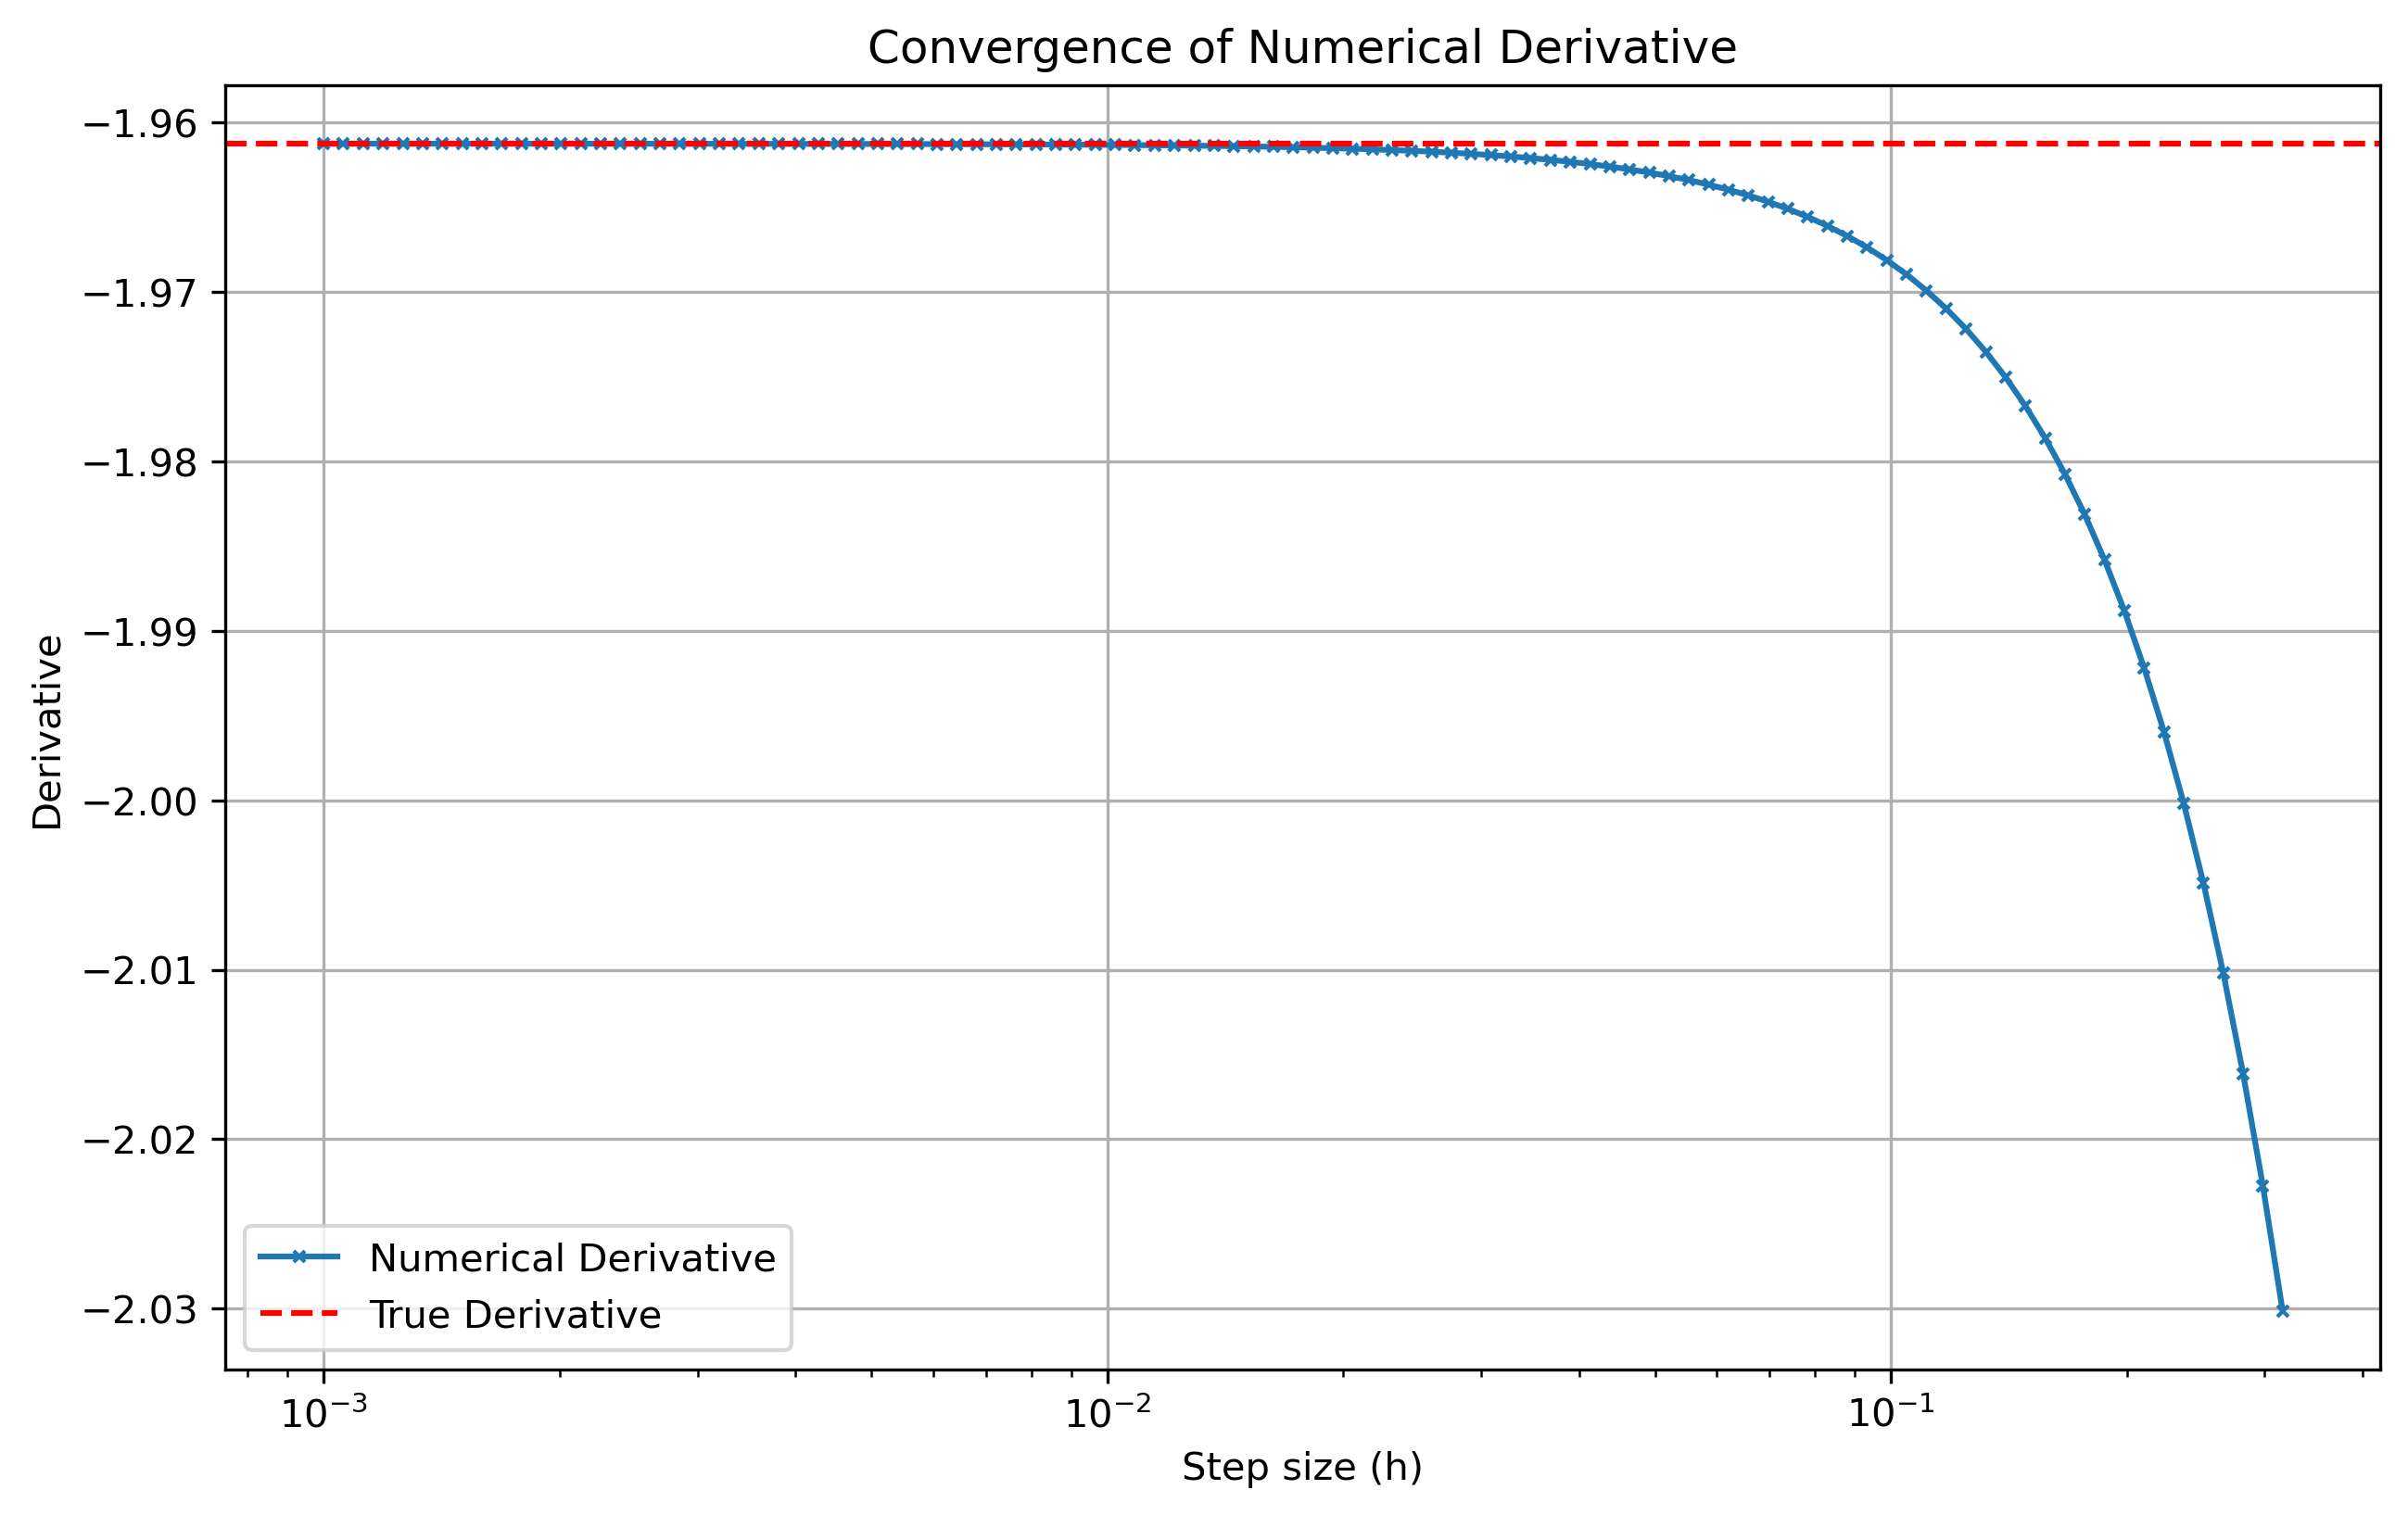
\includegraphics[width=0.8\textwidth]{convergence_derivative.png}
    \caption{Numerical derivative for increasing step sizes (h). The red dashed line indicates the true derivative obtained using dual numbers.}
    \label{fig:convergence_derivative}
\end{figure}

The numerical derivative converges to the true value for small step sizes (approximately \(< 10^{-2}\)) but diverges as \(h\) increases due to round-off errors. In contrast, the dual number method provides a stable and precise derivative, unaffected by the limitations of finite differences. Moreover, dual numbers compute the derivative in a single step, making the method both computationally efficient and less prone to errors.


\section{Tests and Validation}

The \texttt{tests/} directory contains unit tests designed to validate the functionality of the \texttt{dual\_autodiff} package. These tests ensure the correctness of mathematical operations, dual number functionality, and integration with various functions like trigonometric, logarithmic, and exponential operations.

The directory includes the following key test files:
\begin{itemize}
    \item \texttt{test\_dual.py}: Validates the core \texttt{Dual} class, including arithmetic operations and function implementations.
    \item \texttt{test\_functions.py}: Tests global mathematical functions like \texttt{sin}, \texttt{cos}, and \texttt{log}.
    \item \texttt{test\_base.py}: Ensures utility functions such as \texttt{is\_dual\_instance()} and \texttt{ensure\_dual()} work correctly.
\end{itemize}

The tests validate that the \texttt{dual\_autodiff} package functions as expected under various scenarios. They also confirm that dual numbers provide accurate derivatives.
In total 18 tests were created - all passing successfully.


\section{Project Documentation with Sphinx}

The \texttt{dual\_autodiff} package documentation was generated using Sphinx, providing clear explanations, examples, an API reference, and a tutorial notebook.

\subsection{Setup and Configuration}
The \texttt{docs/} directory was created using \texttt{sphinx-quickstart}, which generated configuration files such as \texttt{Makefile}, \texttt{conf.py}, and initial templates for reStructuredText (\texttt{.rst}) files. Key configurations included enabling extensions like \texttt{sphinx.ext.autodoc} (for API generation), \texttt{sphinx.ext.napoleon} (for docstring style), and \texttt{sphinx.ext.viewcode} (for linking code). Additionally, \texttt{nbsphinx} was added to integrate the tutorial notebook.

\subsection{Documentation Structure}
The \texttt{source/} directory contains:
\begin{itemize}
    \item \texttt{index.rst}: Main landing page linking all sections.
    \item \texttt{dual\_autodiff.rst}: Auto-generated API documentation.
    \item \texttt{modules.rst}: Auto-generated list of modules.
    \item \texttt{tutorial.rst}: User guide linked to the tutorial notebook.
    \item \texttt{dual\_autodiff.ipynb}: Notebook showcasing examples and usage.
    \item \texttt{implementation.rst}: Theoretical background and implementation details.
    \item \texttt{apple\_silicon\_x86\_setup.rst}: Setup steps for Apple Silicon devices.
\end{itemize}

\subsection{Generating the Documentation}
HTML documentation was generated by running:
\begin{verbatim}
make html
\end{verbatim}
This compiled the \texttt{.rst} files and \texttt{.ipynb} notebook into structured HTML files in the \texttt{build/html/} directory.

\subsection{Output and Features}
The final documentation includes:
\begin{itemize}
    \item \textbf{Landing Page:} Overview with links to all sections.
    \item \textbf{API Reference:} Detailed documentation of modules and functions.
    \item \textbf{Tutorial Page:} Practical examples and usage guide.
    \item \textbf{Implementation Page:} Theoretical background and key concepts.
\end{itemize}
The integration of \texttt{autodoc} and \texttt{nbsphinx} ensures docstrings from the codebase and the tutorial notebook are included, enhancing accessibility for users.


\section{Cythonizing the Package}

\subsection{Configuration and Implementation}
To Cythonize the \texttt{dual\_autodiff} package, a separate directory named \texttt{dual\_autodiff\_x} was created. This included necessary configurations to ensure efficient compilation and distribution of the Cythonized version.

\subsubsection{Key Configuration Files}
\begin{itemize}
    \item \textbf{\texttt{setup.py}:} Defined Cython modules to be compiled (e.g., \texttt{dual.pyx}, \texttt{functions.pyx}) and metadata for the package.
    \item \textbf{\texttt{pyproject.toml}:} Declared build dependencies (\texttt{Cython}, \texttt{setuptools}, \texttt{wheel}) and Python version compatibility.
    \item \textbf{\texttt{MANIFEST.in}:} Included essential files (\texttt{README.md}, compiled \texttt{.so} files) while excluding unnecessary source files (\texttt{.pyx}, \texttt{.py}).
\end{itemize}

\subsubsection{Cythonization Process}
\begin{enumerate}
    \item \textbf{Code Preparation:} 
    Python files (\texttt{.py}) in the original \texttt{dual\_autodiff} directory were copied into \texttt{dual\_autodiff\_x} and renamed to \texttt{.pyx} to allow Cython compilation.
    
    \item \textbf{Compilation:} 
    The source files were compiled into shared object files (\texttt{.so}) using:
    \begin{verbatim}
    python setup.py build_ext --inplace
    \end{verbatim}
    
    \item \textbf{Installation:} 
    The package was installed in editable mode for testing and further development:
    \begin{verbatim}
    pip install -e .
    \end{verbatim}
\end{enumerate}

The \texttt{.so} and \texttt{.c} files are excluded from the GitLab repository because they are platform-specific and can be regenerated from the \texttt{.pyx} source files using Cython. Including these files would unnecessarily increase the repository size and could lead to compatibility issues, as the compiled files depend on the system architecture and compiler settings of the development environment.

\section{Performance Insights}
To evaluate the effectiveness of Cythonization, we compared the performance of the pure Python and Cythonized implementations.

\subsection{Experimental Setup}
Execution times were measured for arrays of dual numbers with lengths ranging from 100 to 14,000. Three ranges of real parts were considered: \((0,10)\), \((10,100)\), and \((100,1000)\). Each experiment was repeated 100 times, and linear regression was applied to analyse gradients of execution time with respect to array length.

\subsection{Observations}
Figure~\ref{fig:performance_comparison} illustrates the performance comparison:
\begin{itemize}
    \item The Cythonized version exhibited lower execution times across all scenarios.
    \item Gradients for the Cythonized implementation were consistently smaller, highlighting better scalability.
    \item Performance improvements were particularly notable for larger arrays, validating the computational efficiency of Cython.
\end{itemize}

\begin{figure}[h!]
    \centering
    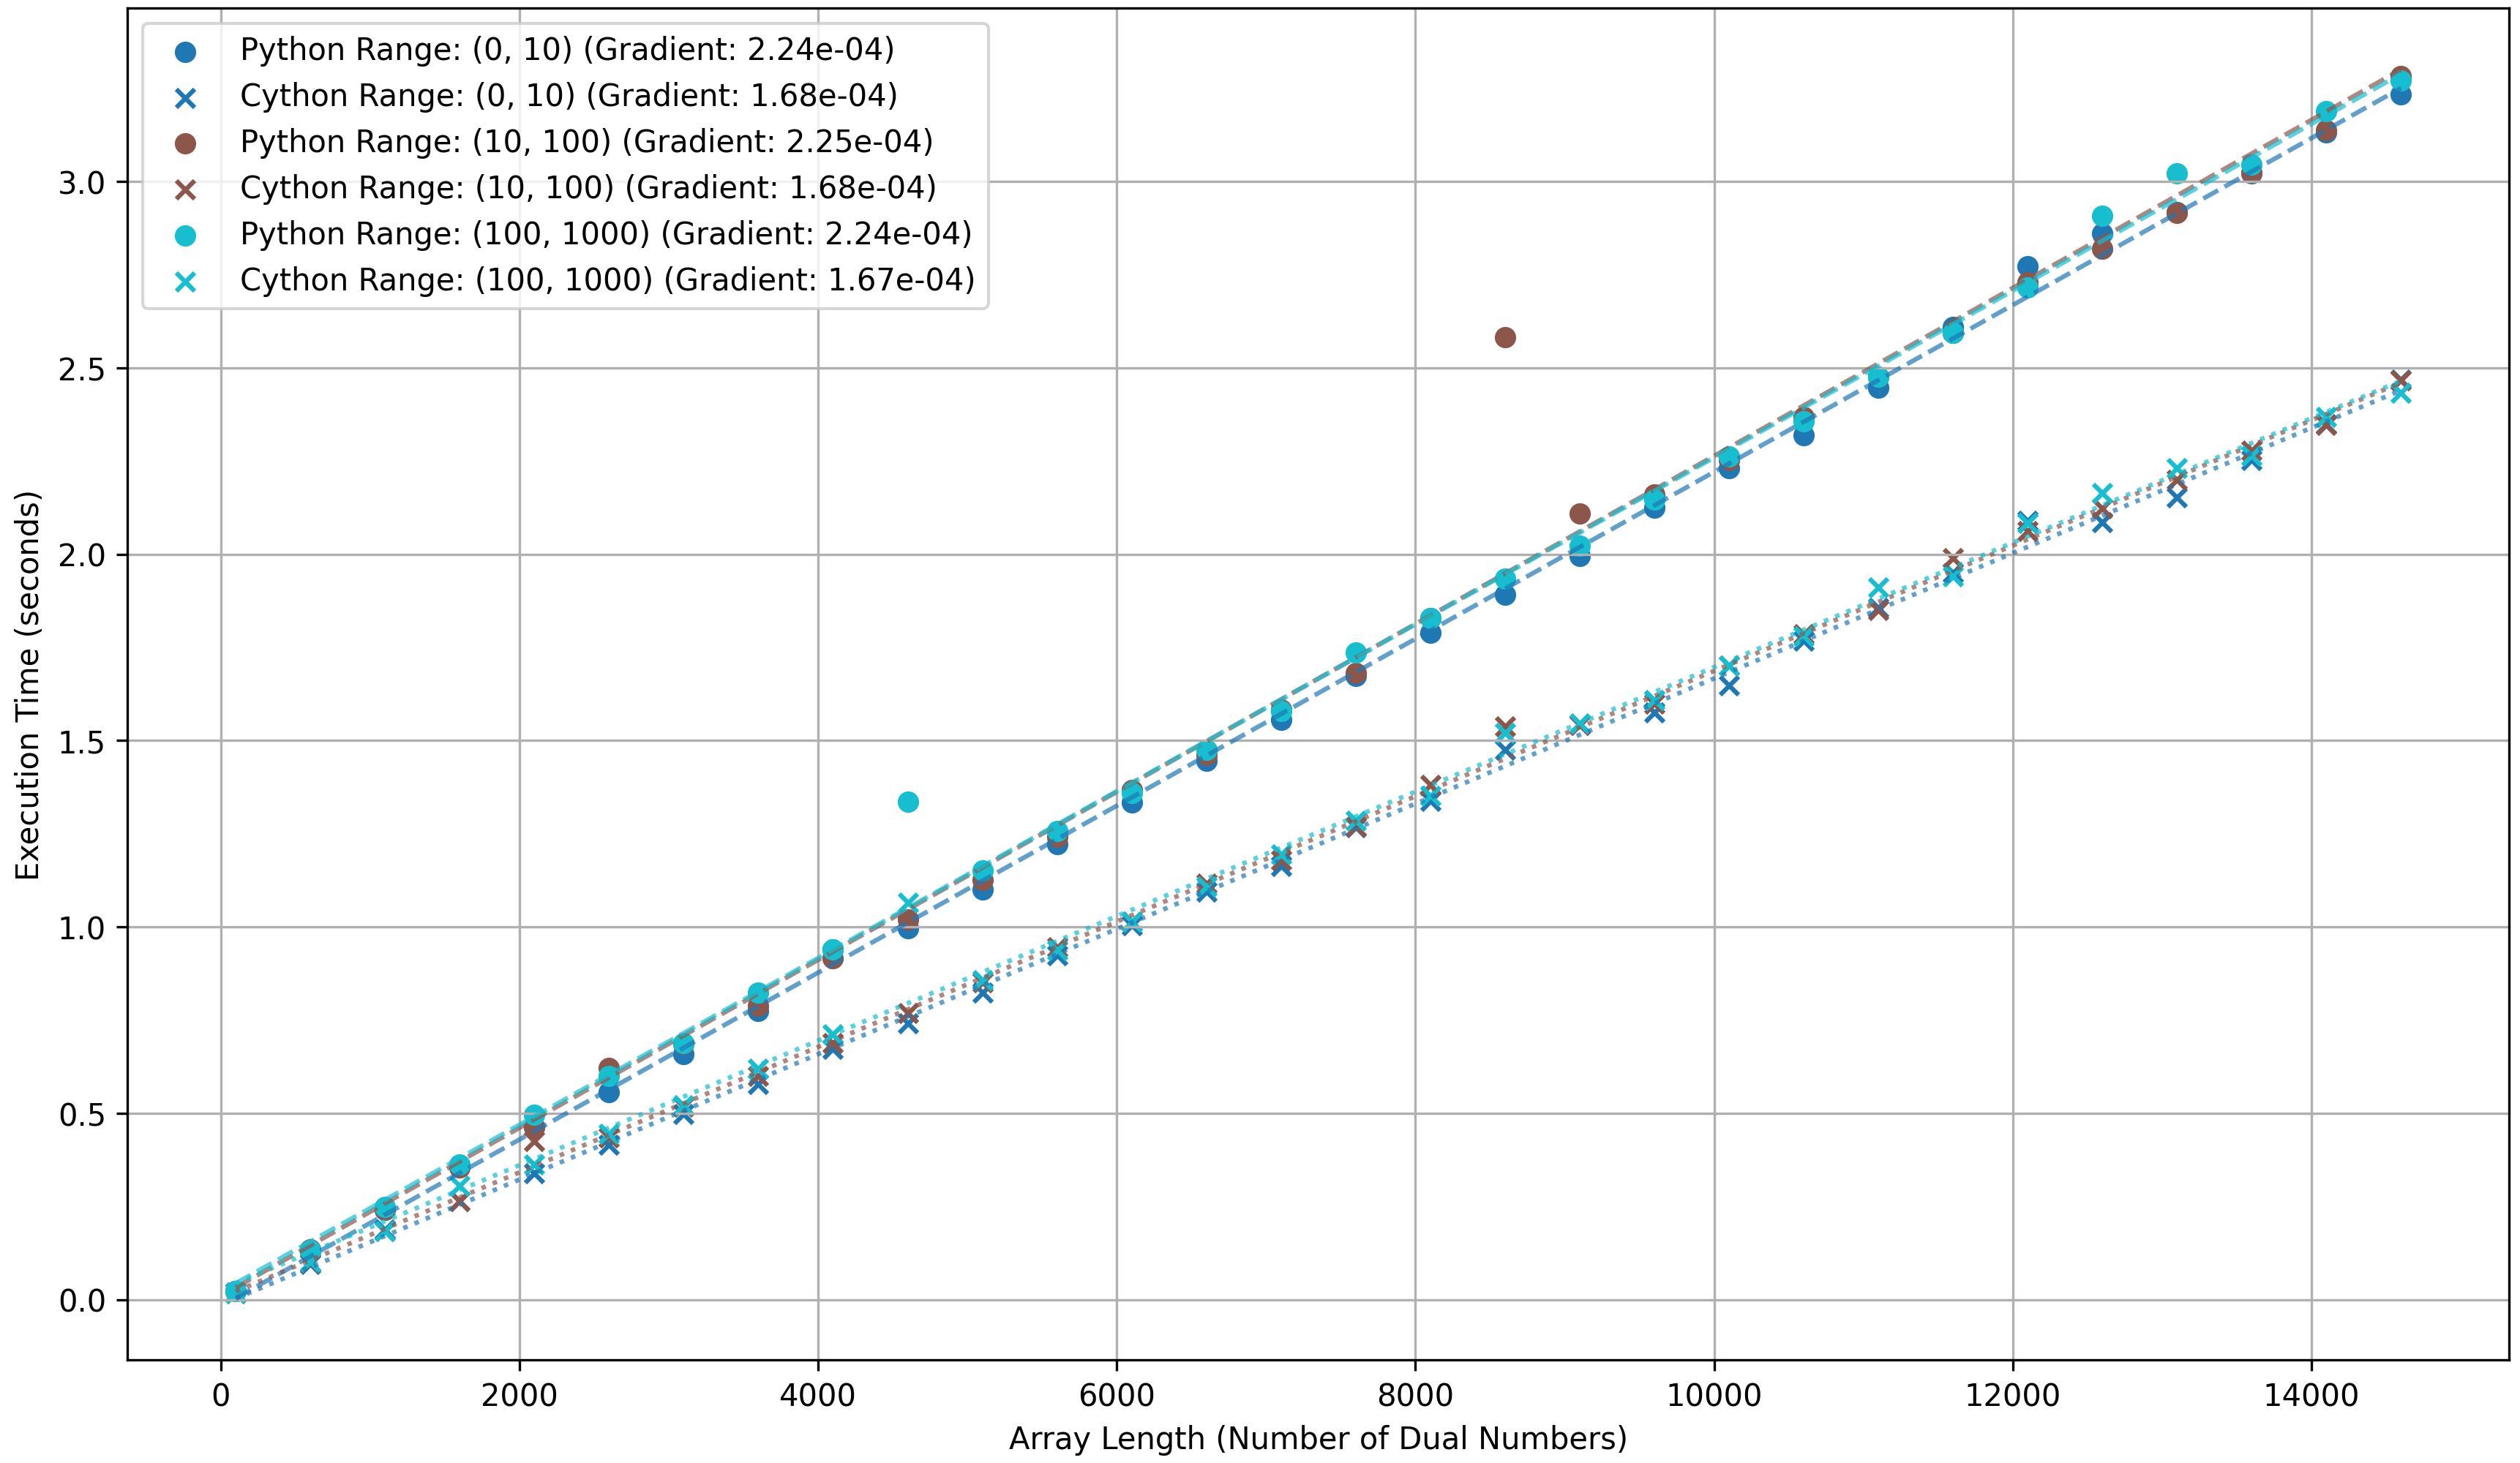
\includegraphics[width=0.8\textwidth]{performance_comparison.png}
    \caption{Performance comparison between the pure Python and Cythonized versions of \texttt{dual\_autodiff}. The gradients indicate the rate of increase in execution time with array length.}
    \label{fig:performance_comparison}
\end{figure}

Figure~\ref{fig:performance_comparison} shows how execution time scales with array length. Python implementation gradients are higher (\(2.20 \times 10^{-4}\)), showing faster growth in execution time, unaffected by the range of real parts. In contrast, Cythonized gradients (\(1.63 \times 10^{-4}\)) are lower, showing better scalability and suitability for larger datasets.

\subsection{Conclusion}
Cythonization improves the scalability and efficiency of the \texttt{dual\_autodiff} package by converting Python code into optimised C extensions. The reduced overhead and compiled nature of Cython minimise dynamic type-checking, leading to lower execution times and better handling of computationally intensive tasks.

Applications like machine learning, requiring differentiation of large parameter arrays, and computational physics, involving derivatives of discretised data points, benefit from this improved performance. Faster computation reduces runtime and resource usage, making the Cythonized version ideal for large-scale problems.

These results align with prior studies~\cite{mortensen2016cython}, demonstrating that Cython achieves performance comparable to low-level languages like C++. The findings validate the advantages of Cythonization for real-world, high-performance applications.


\section{Building Wheels for Linux}

To create specific wheels for the \texttt{dual\_autodiff\_x} package targeting \texttt{cp310-manylinux\_x86\_64} and \texttt{cp311-manylinux\_x86\_64}, I initially attempted the process manually on the University of Cambridge's CSD3 cluster due to compatibility issues on macOS M4. Later, I used a family member's laptop, which allowed me to generate wheels in the required manylinux format with a single command.

The initial steps on CSD3 taught me valuable lessons about creating environments, understanding computer architecture, and troubleshooting compatibility challenges. Although these steps produced linux-compatible wheels, not produce manylinux-compatible wheels, the experience deepened my technical understanding and problem-solving skills. Borrowing an older laptop ultimately provided a simpler and more effective solution.


By utilising a family member's laptop, I generated both wheels in the \texttt{manylinux} format with a single command:
\begin{verbatim}
CIBW_BUILD="cp310-manylinux_x86_64 cp311-manylinux_x86_64" cibuildwheel
 --output-dir wheelhouse
\end{verbatim}
The \texttt{CIBW\_BUILD} environment variable specifies that the wheels should be built exclusively for Python 3.10 and Python 3.11 on the \texttt{manylinux\_x86\_64} platform. This command uses \texttt{cibuildwheel}, which employs Docker (running in the background) to efficiently build compatible wheels, outputting the generated wheels to the \texttt{wheelhouse/} directory.

The resulting wheels were named:
\begin{itemize}
    \item rsr45\_dual\_autodiff\_x-0.1.16-cp310-cp310-manylinux\_2\_17\_x86\_64.manylinux2014\_x86\_64.whl
    \item rsr45\_dual\_autodiff\_x-0.1.16-cp311-cp311-manylinux\_2\_17\_x86\_64.manylinux2014\_x86\_64.whl
\end{itemize}

The naming convention of the wheels is determined automatically by \texttt{cibuildwheel}:
\begin{itemize}
    \item \textbf{Package Name:} \texttt{rsr45\_dual\_autodiff\_x}, which uniquely identifies the package.
    \item \textbf{Version:} \texttt{0.1.16}, reflecting the current version of the package.
    \item \textbf{Python Tag:} \texttt{cp310} and \texttt{cp311}, denoting compatibility with Python 3.10 and 3.11.
    \item \textbf{ABI Tag:} Repeated \texttt{cp310} or \texttt{cp311}, indicating compatibility with the specific Python Application Binary Interface (ABI).
    \item \textbf{Platform Tag:} \texttt{manylinux\_2\_17\_x86\_64.manylinux2014\_x86\_64}, signifying compliance with the \texttt{manylinux2014} standard for Linux distributions.
\end{itemize}



The wheels are stored in the \texttt{wheelhouse/} directory, and their contents were verified by extracting each into the \texttt{wheel\_contents/} directory:
\begin{itemize}
    \item \textbf{Compiled Binaries:} Shared object files (\texttt{*.so}) for the core modules (\texttt{base}, \texttt{dual}, \texttt{functions}, and \texttt{version}), compiled for both \texttt{x86\_64-linux-gnu} (manylinux-compatible) and \texttt{darwin} (macOS). These binaries ensure platform compatibility.
    \item \textbf{Metadata:} The \texttt{*dist-info} directory contains essential metadata files, including:
    \begin{itemize}
        \item \texttt{METADATA}: Provides details about the package, such as name, version, and dependencies.
        \item \texttt{WHEEL}: Specifies compatibility standards and wheel-specific metadata.
        \item \texttt{RECORD}: Contains file integrity information, including hashes and file paths.
    \end{itemize}
\end{itemize}



\section*{PyPI Upload}

The \texttt{dual\_autodiff\_x} package was uploaded to PyPI under the name \texttt{rsr45-dual-autodiff-x}, allowing users to install it easily via:
\begin{verbatim}
pip install rsr45-dual-autodiff-x
\end{verbatim}

The package is available at the following link: \href{https://pypi.org/project/rsr45-dual-autodiff-x/}{https://pypi.org/project/rsr45-dual-autodiff-x/}


\section{Uploading Wheels to GitLab Repository}

The \texttt{wheelhouse/} directory contains the wheels built for Python 3.10 and 3.11, specifically targeting the \texttt{cp310-manylinux\_x86\_64} and \texttt{cp311-manylinux\_x86\_64} platforms. To upload these wheels to the GitLab repository, I first ensured they were properly located in the \texttt{dual\_autodiff\_x/wheelhouse/} directory. I then staged the files using \texttt{git add}, committed the changes with a descriptive message indicating the addition of the manylinux wheels, and pushed the changes to a dedicated branch. 

This approach allowed me to validate the wheels and ensure their correctness before merging the branch into the main repository. Once I confirmed the wheels worked as expected and passed all tests, I merged the branch into the main repository, maintaining a reliable and well-documented development history.


\subsection{Installation and Validation}
After downloading the wheels from the GitLab repository, the package can be installed on any Linux system, such as CSD3 or a local laptop, using the following command:
\begin{verbatim}
pip install rsr45_dual_autodiff_x_<name_of_wheel>.whl
\end{verbatim}

The prefix \texttt{rsr45} in the wheel name reflects the unique naming convention required to identify this package as part of my coursework submission, distinguishing it from any existing or similarly named packages on PyPI or other systems. This ensures that the package is easily attributable to me and avoids potential conflicts with other versions of \texttt{dual\_autodiff\_x}.

To verify the installation, the examples provided in the tutorial notebook \texttt{dual\_autodiff.ipynb} were executed. 




\section{Conclusion}

This project successfully developed the \texttt{dual\_autodiff} package, implementing forward-mode automatic differentiation using dual numbers. Key objectives, including creating the \texttt{Dual} class, enhancing performance through Cythonization, and packaging with \texttt{cibuildwheel}, were accomplished. The resulting packages, \texttt{rsr45-dual-autodiff} and \texttt{rsr45-dual-autodiff-x}, are publicly available on PyPI for easy installation and use.

The Python implementation prioritised ease of use, while the Cythonized version (\texttt{dual\_autodiff\_x}) improved performance which was quantitatively evaluated. Best practices, such as unit testing, detailed documentation via Sphinx, and a tutorial notebook, ensured the package's robustness and practical applicability.

This coursework strengthened skills in computational physics, software optimisation, and problem-solving. Future work could expand the package to support higher-order derivatives, alternate differentiation modes, and additional architectures, such as ARM-based platforms. Overall, the \texttt{dual\_autodiff} package is a versatile tool with applications in optimisation, machine learning, and computational physics.

\printbibliography

\section*{Declaration of Use of AI Tools}

I declare that all ideas, methods, and approaches used in this project were conceived and developed independently through my own research, understanding and engagement with lecture and supervision material. The work presented here is entirely my own.

The following AI tools were used for support purposes:
\begin{itemize}
    \item \textbf{ChatGPT:} Used to refine code snippets, assist with LaTeX formatting, and improve the clarity and structure. All content generated by this tool was critically evaluated and adapted.
    \item \textbf{GitHub Copilot:} Used to suggest coding snippets and assist the implementation of functions. All suggested code was reviewed, modified, and tested.
\end{itemize}

\end{document}
